%\documentclass[a4paper]{article}
\documentclass[12pt]{report}

\usepackage[paper=a4paper,dvips,top=2.5cm,left=2cm,right=2cm,
    foot=1cm,bottom=3cm]{geometry}
\usepackage{titlesec}
\titleformat{\chapter}[hang]
{\normalfont\huge\bfseries}{\chaptertitlename\ \thechapter.}{.4em}{}

\usepackage[english]{babel}
\usepackage[utf8]{inputenc}
\usepackage{amsmath}
\usepackage{cases}
\usepackage{amsfonts}
\usepackage{graphicx}
\usepackage{array}
\usepackage{mathtools}
\usepackage{caption}
\usepackage{float}
\usepackage[framed, numbered]{mcode}
\usepackage{subcaption}
\usepackage{epstopdf}
\usepackage{framed}
\usepackage{courier}
\usepackage[T1]{fontenc}
\usepackage[]{algorithm2e}
\usepackage{sidecap}
\usepackage[colorinlistoftodos]{todonotes}
\usepackage{natbib}
\usepackage{url}
\usepackage{booktabs}

\title{Partial differential equation based image processing and applications}
\author{Euijae Kim}
\date{\today}

\begin{document}
    % --------------- %
	% HERE IS A TITLE %
    % --------------- %
	\maketitle
    % ----------------- %
	% HERE IS A SECTION %
    % ----------------- %
    \section*{Abstract}
Image processing represents images as matrices or 2D arrays. Each entry is called a pixel; each pixel has a value and represents a color. Just like how people can identify other people, objects, and places within a picture, machines can also recognize a person, thing, or place within a picture. More precisely, machines try to detect these images by identifying pixels belonging to an object of interest. From on this basic mechanism, image processing can remove noise, recognize what people search for within the picture, and detect edges. \newline

I present three algorithms for restoration of noisy images. Each algorithm is based on solving an optimization problem via gradient descent partial differential equations. The three algorithms correspond to the heat equation, the Rudin-Osher-Fatemi total variation restoration, and the Perona-Malik anisotropic diffusion equation. Comprehensive examples of each algorithms applied to real noisy images are also shown and the performance is analyzed in terms of PSNR.
    % ----------------- %
	% HERE IS ACKNOWLEG %
    % ----------------- %
    \section*{Acknowledgements}
Sincere thanks to my parents and Prof. Jeff Calder.

    % ----------------------- %
	% HERE IS LIST OF FIGURES %
    % ----------------------- %
	\listoffigures
    % ----------------- %
	% HERE IS A CONTENT %
    % ----------------- %
	\begin{tableofcontents}
		% ------------------------------- %
    	% HERE IS A CH2(IMAGE PROCESSING) %
        % ------------------------------- %
        \chapter{Image Processing}
			% ---------------------- %
			\section{Basic Mechanisms}
			% ---------------------- %
We see a picture. In it, there are friends, family, famous landmarks, and other significant images. They are what we try to record and remember. In short, we mostly focus on three characteristics: who, what, and where. Although machines can also recognize the defining qualities of an image, their processes of recognition differ significantly from ours. Analyzing the pixels belonging to an object of interest is, essentially, how a machine can decipher image content. From a scientific point of view, machines try to remove noise and detect edges or objects. Finally, the machines store and present these deciphered images. In the core of this paper, I will not only present some image processing algorithms for denoising, but I will also analyze the performance of each algorithm on a test image.
        	\begin{figure}[ht]
				\centering
				\begin{subfigure}{0.3\textwidth}
					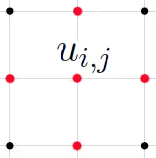
\includegraphics[width=\textwidth]{stencils.png}
					%\caption{Two dimensional}
				\end{subfigure}
				\caption{Structure of Grayscale image matrix}
			\end{figure}
\newline
\par
All digital image processing represents images as a matrix or 2D array. With grayscale image, we model images as function $u:\Omega \to [0,1]$ where $\Omega = [0,1]^2$ denote the image domain, and $u(x,y)$ denotes the intensity or brightness of the image where $x,y$ represents locations. On a computer, we can store a discrete version of $f$, sampled on a uniform two dimensional grid, and process the discrete or digital version of the image. In Matlab, this two dimensional array is organized into a matrix. For color images, we model images as function $u:\Omega \to [0,1]^3$, where $u(x,y)$ is now a vector in $\mathbb{R}^3$ consisting of the RGB values of the image at location $(x,y)$. This vector can also contain YUV values or values from any other color space. In Matlab, these data are organized into a three dimensional array of size $M\times N\times$ 3. I will only perform floating point precision arithmetic on each image processing algorithm.
        	\begin{figure}[ht]
				\centering
				\begin{subfigure}{0.24\textwidth}
					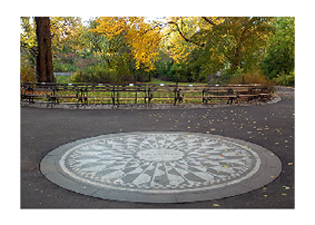
\includegraphics[width=\textwidth]{rgb_ori.png}
					\caption{Original Image}
				\end{subfigure}
				\begin{subfigure}{0.24\textwidth}
					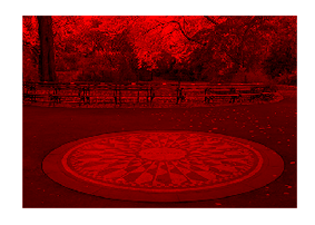
\includegraphics[width=\textwidth]{rgb_r.png}
					\caption{Red Channel}
				\end{subfigure}
				\begin{subfigure}{0.24\textwidth}
					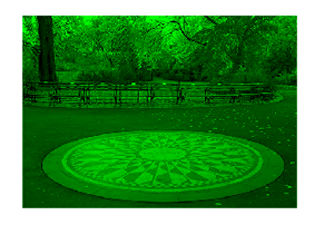
\includegraphics[width=\textwidth]{rgb_g.png}
					\caption{Green Channel}
				\end{subfigure}
				\begin{subfigure}{0.24\textwidth}
					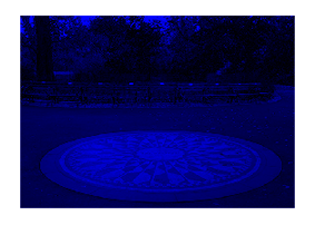
\includegraphics[width=\textwidth]{rgb_b.png}
					\caption{Blue Channel}
				\end{subfigure}
				\caption{Each Channels of RGB}
			\end{figure}
            % ----------- %
            \section{Noise}
            % ----------- %
Image noise refers to random variations in brightness or color information within images. I will introduce processes illustrating the denoising of these images in \textbf{Chapter 2}. Mathematically, we model noise using random variables. Let $u:\Omega \to [0,1]$ denote a grayscale image. We consider additive noise to be of the form
			\begin{alignat*}{1}
		u_{N}(x,y) &= u(x,y) + \eta(x,y)
        	\end{alignat*}
where $\eta(x,y)$ is a random variable for each $(x,y) \in \Omega$ and $u_{N}$ denotes the noisy image. We consider additive Gaussian noise, which is obtained by taking $\eta(x,y)$ to be a Gaussian random variable of standard deviation $\sigma$ for each $(x,y)$. Then this is implemented in Matlab as follows:
\begin{lstlisting}
f = imread(Image); % Convert to matrix
f = im2double(f);  % Cast value type to double
[row, col, channel] = size(f); % Take size of f
Noise = f + 0.1*randn(row, col, channel); % Create a noise image
\end{lstlisting}
			\begin{figure}[ht]
				\captionsetup[subfigure]{labelformat=empty}
				\centering
				\begin{subfigure}{0.49\textwidth}
					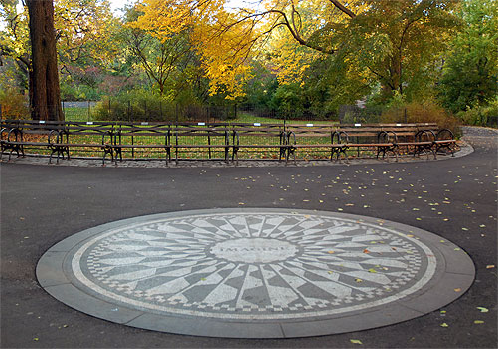
\includegraphics[width=\textwidth]{noise_00.png}
					\caption{(a) $\sigma$=0.00, Original image}
				\end{subfigure}
				\begin{subfigure}{0.49\textwidth}
					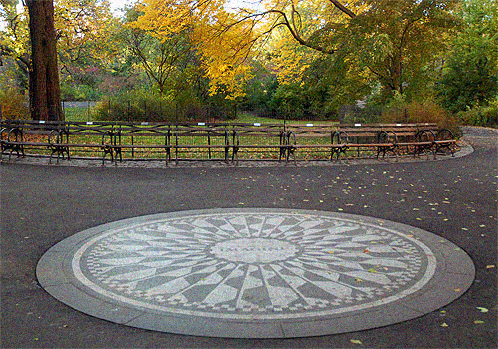
\includegraphics[width=\textwidth]{noise_05.png}
					\caption{(b) $\sigma$=0.05}
				\end{subfigure}
			\end{figure}
            \begin{figure}[ht]
				\captionsetup[subfigure]{labelformat=empty}
                \centering
				\begin{subfigure}{0.49\textwidth}
					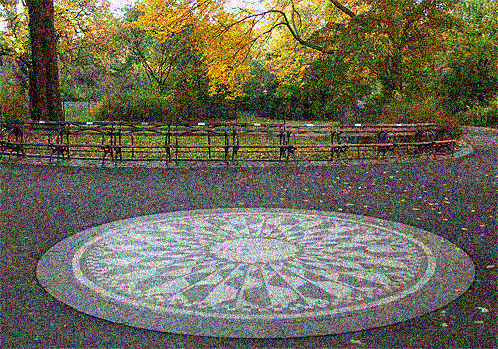
\includegraphics[width=\textwidth]{noise_15.png}
					\caption{(c) $\sigma$=0.15}
				\end{subfigure}
				\begin{subfigure}{0.49\textwidth}
					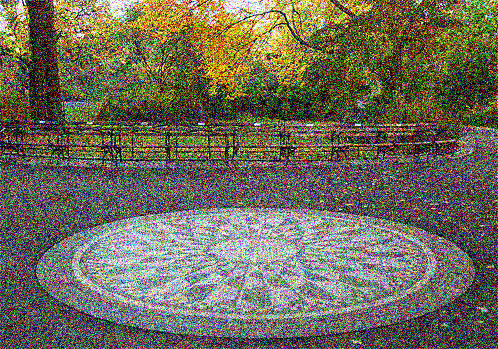
\includegraphics[width=\textwidth]{noise_25.png}
					\caption{(d) $\sigma$=0.25}
				\end{subfigure}
				\caption{Noise increasing as $\lambda$ gets bigger}
			\end{figure}

            % ---------- %
			\section{Blur}
            % ---------- %
A blurred image can result from either motion of camera as it operates or improper focal distancing, among other reasons. For a blurring kernel $h$, blur is defined as
			\begin{alignat*}{1}
            f_{B}(x,y) &= \int_{-\infty}^{\infty} h(x-s, y-t)\cdot f(s,t)ds dt
            \end{alignat*}
\par
The Matlab command \textbf{fspecial} provides various types of blur kernels. With this kernel, and the command \textbf{imfilter}\cite{imfilter}, the image can be blurred. For example, the code below blurs an image of the Strawberry Field in Central Park, NY. The keyword 'motion' returns a filter that, once combined with the image, approximates the linear motion of a camera by lens pixels, where the camera moves an angle of theta degrees in a counterclockwise direction. The filter is a vector representing horizontal and vertical motion. For the kernel $h$ defined above, it can be formed by matrix where black has a value of 0 as follows:
			\begin{figure}[H]
				\centering
				\begin{subfigure}{0.7\textwidth}
					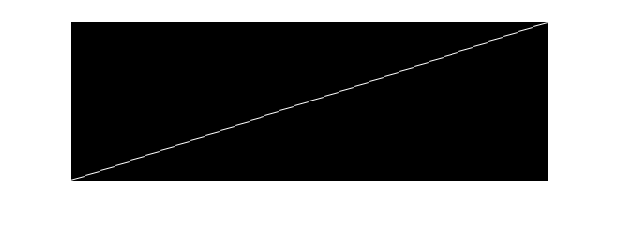
\includegraphics[width=\textwidth]{kernel.png}
				\end{subfigure}
                \caption{Behave of kernel $h$}
			\end{figure}
\noindent
We consider in this paper motion blur, implemented in Matlab as follows:
\begin{lstlisting}
f = imread(Image);
h = fspecial('motion', 15, 15);
b = imfilter(f, h, 'replicate');
\end{lstlisting}
        	\begin{figure}[H]
				\centering
				\captionsetup[subfigure]{labelformat=empty}
				\begin{subfigure}{0.49\textwidth}
					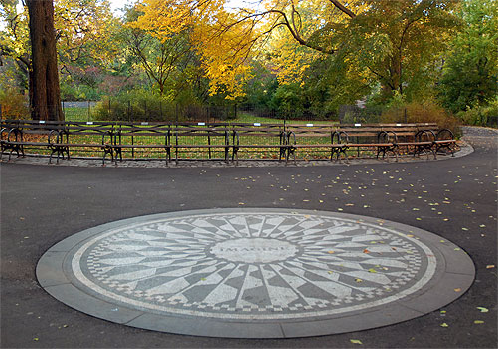
\includegraphics[width=\textwidth]{original.png}
					\caption{(a) Original image}
				\end{subfigure}
				\begin{subfigure}[h]{0.49\textwidth}
					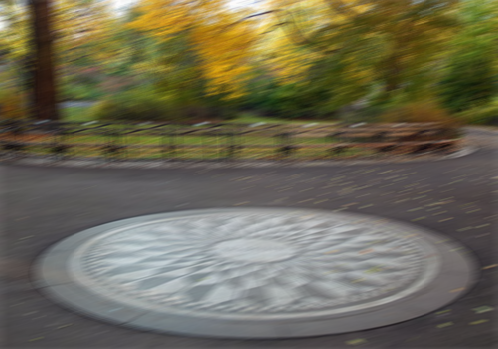
\includegraphics[width=\textwidth]{blurr.png}
					\caption{(b) Blurred image}
				\end{subfigure}
				\caption{Blurred image}
			\end{figure}


		% ---------------------------------------------------- %
    	% HERE IS A PDE										   %
        % ---------------------------------------------------- %
		\chapter{Partial Differential Equations}
Let $f:\Omega \to [0,1]$ be an image that has been corrupted by noise. The noisy image is restored by seeking to find an image u that minimizes the energy $E[u]$ given by the following equation
%Then I restore the noisy image by seeking to find an image $u$ that minimizes energy $E[u]$ follows over all such image
\newline
			\begin{equation}
E\left[u\right] = \displaystyle\min_{u}\frac{1}{2} \int_\Omega \phi(|\nabla u|^2) \, dx dy + \frac{\lambda}{2}\int_{\Omega}(u-f)^2 dxdy
			\end{equation}
The energy function $E[u]$ has two terms as can be seen from its expression. The first term is free of noise and hence, makes $E[u]$ smooth while the second term is fidelity term and hence, introduces the noise in the image. There are different algorithms for denoising or restoring images and are based on $E[u]$ for different choices of $\phi$. Since these three can be interpreted as gradient descent equations for the function $E$, the schemes will be implemented based on gradient descent equations and $E[u]$.
%where $E[u]$ refers to the energy itself, and should not have $\displaystyle\min_{u}$ in the definition. The 1st term in $E[u]$ is a prior that encourages $u$ to be smooth and free of noise, while the 2nd term is a fidelity term that encourages $u$ to resemble the noisy image $f$.
\newline
\newline
Let $g(u, u_{x}, u_{y})=\phi(|\nabla u|^2) \, + \frac{\lambda}{2}(u-f)^2$. Then introduce  $\nabla E$ that behaves like gradient and $E[u]$ has a extrema where $\nabla E$=0. Furthermore, $\nabla E$ points in the direction of maximum positive rate of change. Note that $|\nabla u|^2=u_{x}+u_{y}$. By Euler-Lagrange equation,
			\begin{alignat*}{5}
\nabla E &= \frac{\partial}{\partial u} - \frac{\partial}{\partial x}\frac{\partial g}{\partial u_{x}}
			- \frac{\partial}{\partial y}\frac{\partial g}{\partial u_{y}} \\
	&= \lambda(u-f) - \frac{\partial}{\partial x}\frac{1}{2}\phi'(u_{x}^2+u_{y}^2)2u_{x}
    	- \frac{\partial}{\partial y}\frac{1}{2}\phi'(u_{x}^2+u_{y}^2)2u_{y} \\
	&= \lambda(u-f) - \frac{\partial}{\partial x}\phi'(u_{x}^2+u_{y}^2)u_{x}
    	- \frac{\partial}{\partial y}\phi'(u_{x}^2+u_{y}^2)u_{y} \\
	&= -\lambda(f-u) - \text{div}\Big(\phi'(u_{x}^2+u_{y}^2)(u_{x}+u_{y})\Big) \\
    &= -\Big[\lambda(f-u) + \text{div}\Big(\phi'(|\nabla u|^2)(\nabla u)\Big)\Big]
            \end{alignat*}
To find $\displaystyle\min_{u}E[u]$, let $\Delta t$ be a small step size in the direction of $-\nabla E$ and then
			\begin{equation}
u_{i,j}^{n+1} = u_{i,j}^{n} + \Delta t(-\nabla E)
			\end{equation}
This equation can be modified as
			\begin{equation}
            \begin{split}
\displaystyle\frac{\partial u}{\partial t}
		&= \text{div}\Big( \phi'(|\nabla u|^{2})\nabla u\Big) + \lambda (f-u)\\
		&= -\nabla E
        	\end{split}
			\end{equation}
The last equation represents the gradient descent. The gradient descent for heat equation, Perona-Malik, and total variation are determined by different choices of $\phi$, which is as follows:
\[ \left\{
  \begin{array}{l l}
    \phi(s)=s & \quad \text{Heat Equation}\\
    \phi'(s)=c(s) & \quad \text{Perona-Malik. c is flux function, detailed in \textbf{Chapter 2.2}} \\
    \phi(s)=\sqrt{s} & \quad \text{total variation}
  \end{array} \right.\]
			% ------------------- %
			\section{Heat Equation}
			% ------------------- %
As described above, heat equation takes $\phi(s)=s$. By Taylor's expansion, we can expand $u(x+h)$ $\text{and}$ $u(x-h)$ as follows:
				\begin{equation}
                \begin{split}
\displaystyle u(x+h) &= u(x) + hu'(x) + \frac{h^2}{2}u''(x) + O(h^3) \\
\displaystyle u(x-h) &= u(x) - hu'(x) + \frac{h^2}{2}u''(x) + O(h^3)
				\end{split}
				\end{equation}
Adding two equations in (2.3) follows that
				\begin{alignat*}{1}
\displaystyle u(x+h) + u(x-h) = 2u(x) + h^2u''(x) + O(h^3)
				\end{alignat*}
%Then we can have a following equation when solving for $u''$
Solving for u’’, the following equation is obtained
				\begin{equation}
u''(x) = \frac{1}{h^2}\Big[u(x+h) - 2u(x) + u(x-h)\Big] + O(h)
                \end{equation}
\newline
Based on (2.4), because $u$ was defined as multivariable function in $x$ and $y$, approximation of $\Delta u$ is
				\begin{equation}
                \begin{split}
      \displaystyle\Delta u &\approx \frac{u_{i+1,j}-2u_{i,j}+u_{i-1,j}}{h^2}+\frac{u_{i,j+1}-2u_{i,j}+u_{i,j-1}}{h^2}\\
              &\approx \frac{1}{h^2}(u_{i+1,j}+u_{i-1,j}+u_{i,j+1}+u_{i,j-1}-4u_{i,j})
              	\end{split}
                \end{equation}
This is the standard 5-point stencil for the Laplacian. The gradient descent for heat equation is given by
				\begin{alignat*}{1}
                \frac{\partial u}{\partial t} &= \Delta u + \lambda(f-u)
                \end{alignat*}
So the equation (2.2) can be modified as
				\begin{alignat*}{1}
                \displaystyle u_{i,j}^{n+1} &= u_{i,j}^{n} + \Delta t\big(u_{i+1,j}+u_{i-1,j}+u_{i,j+1}+u_{i,j-1}-4u_{i,j} + \lambda(f-u)\big)
                \end{alignat*}
\newline
\noindent
The scheme is stable when $\Delta t \leq 0.25$. Note that it is well-known that the heat equation excessively blurs edges and removes important image details.
            \begin{figure}[H]
				\centering
				\begin{subfigure}{0.2\textwidth}
					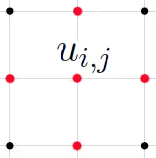
\includegraphics[width=\textwidth]{stencils.png}
				\end{subfigure}
				\caption{Five stencils for heat equation. Red represents used stencils for heat equation}
			\end{figure}
            % --------------------------- %
        	\section{Perona-Malik Equation}
            % --------------------------- %
Perona-Malik propose to perform edge detection and noise removal via anisotropic diffusion \cite{perona1990scale}. Based on the equation (2.2), gradient descent is determined by $\lambda=0$ and $\phi'(s)=c(s)$ where c is the flux function which is chosen locally as a function of a magnitude of the gradient of the image and defined as follows:
\[ c(|\nabla u|) = \left\{
  \begin{array}{l l}
    \text{exp}(-|\nabla u|^{2}/k^{2}) & \quad \text{exponential}\\
    \big(1 + |\nabla u|^2/k^2\big)^{-1} & \quad \text{fractional}
  \end{array} \right.\]
where $k$ is a constant. The simplified divergence operator is given by
			\begin{equation}
            \begin{split}
\displaystyle\frac{\partial u}{\partial t} &= \text{div}\Big(c\big(|\nabla u|^{2}\big)\nabla u\Big) \\
 &= \frac{\partial}{\partial x}\Big(c(x, y, t)u_{x}\Big)
												+ \frac{\partial}{\partial y}\Big(c(x, y, t)u_{y}\Big) \\
 &= \underbrace{c_{x}u_{x} + c_{y}u_{y}}_{(A)} + \underbrace{c(u_{xx} + u_{yy})}_{(B)}
 			\end{split}
            \end{equation}
(A) is discretized using centered differences.
%We discretize (A) using centered differences.
			\begin{equation}
            \begin{split}
c_{x}u_{x}+c_{y}u_{y}
&= \frac{c_{x}}{2}(u_{i+1,j}-u_{i-1,j}) + \frac{c_{y}}{2}(u_{i,j+1}-u_{i,j-1}) \\
&= \frac{c_{x}}{2}(u_{i+1,j}-u_{i,j}+u_{i,j}-u_{i-1,j})
	+\frac{c_{y}}{2}(u_{i,j+1}-u_{i,j}+u_{i,j}-u_{i,j-1})
    		\end{split}
			\end{equation}
where $u_{x}\approx\frac{1}{2}(u_{i+1,j}-u_{i-1,j})$ and $u_{y}\approx\frac{1}{2}(u_{i,j+1}-u_{i,j-1})$
\newline
\newline
For (B), we use the five point stencil for the Laplacian is used.
			\begin{equation}
            \begin{split}
c(u_{xx} + u_{yy})
&= c_{i,j}(u_{i+1,j}+u_{i-1,j}-2u_{i,j}+u_{i,j+1}+u_{i,j-1}-2u_{i,j}) \\
&= c_{i,j}(u_{i+1,j}-u_{i,j}+u_{i-1,j}-u_{i,j}+u_{i,j+1}-u_{i,j}+u_{i,j-1}-u_{i,j})
			\end{split}
            \end{equation}
Defining the vectors
            \begin{alignat*}{4}
            \begin{split}
            \overrightarrow{N} &= u_{i-1,j} - u_{i,j} \\
            \overrightarrow{S} &= u_{i+1,j} - u_{i,j} \\
            \overrightarrow{E} &= u_{i,j+1} - u_{i,j} \\
            \overrightarrow{W} &= u_{i,j-1} - u_{i,j} \\
            \end{split}
            \end{alignat*}
and applying the vectors to the flux equation,
\[ c_{v} = \left\{
  \begin{array}{l l}
    \text{exp}(-v^{2}/k^{2}) & \quad \text{exponential}\\
    \big(1 + v^{2}/k^{2}\big)^{-1} & \quad \text{fractional}
  \end{array} \right.\]
where $v \in \{\overrightarrow{N}, \overrightarrow{S}, \overrightarrow{E}, \overrightarrow{W}\}$ and $N, W, E,\text{and } S$ represent pixel above, left, right, below when it comes to an image matrix space. Then using equations (2.8) and (2.9), the gradient descent is now modified as
			\begin{multline*}
c_{x}u_{x} + c_{y}u_{y} + c(u_{xx} + u_{yy})
= (\overbrace{c_{i,j}+\frac{c_{x}}{2}}^{c_{S}})(\overbrace{u_{i+1,j}-u_{i,j}}^{\overrightarrow{S}})
+ (\overbrace{c_{i,j}-\frac{c_{x}}{2}}^{c_{N}})(\overbrace{u_{i-1,j}-u_{i,j}}^{\overrightarrow{N}})\\
+ (\underbrace{c_{i,j}+\frac{c_{y}}{2}}_{c_{E}})(\underbrace{u_{i,j+1}-I_{i,j}}_{\overrightarrow{E}})
+ (\underbrace{c_{i,j}-\frac{c_{y}}{2}}_{c_{W}})(\underbrace{u_{i,j-1}-u_{i,j}}_{\overrightarrow{W}})
            \end{multline*}
A 4-nearest neighbors discretization of the Laplacian operator which is suggested by Perona-Malik is
			\begin{alignat*}{1}
u_{i,j}^{t+1} = u_{i,j}^{t} + \mu\Big[c_{N}\overrightarrow{N}
			+c_{S}\overrightarrow{S}
            +c_{E}\overrightarrow{E}
            +c_{W}\overrightarrow{W}\Big]_{i,j}^{t}
            \end{alignat*}
where $0 \leq \mu \leq 0.25$ for stability of numerical schemes \cite{perona1990scale}.
            % --------------------- %
        	\section{Total variation}
            % --------------------- %
Rudin, Osher, and Fetami proposed to restore the noisy image $f$ by using $\phi(s)=\sqrt{s}$. Then gradient (2.3) for total variation are modified as follows:
				\begin{alignat*}{2}
	\displaystyle\frac{\partial u}{\partial t}
    		&= \text{div}\Big(\frac{\nabla u}{|\nabla u|}\Big) + \lambda(f-u)
        		\end{alignat*}
where $\lambda$ be a positive parameter \cite{getreuer2012rudin, rudin1992nonlinear}.
Now take $u(0,x) = u_{0}(x)$ be the initial image on $\Omega\times\{t=0\}$. Let $u_{x}=\frac{\partial u}{\partial x}$ and $u_{y}=\frac{\partial u}{\partial y}$. Then expanding the divergence,
				\begin{alignat*}{1}
\text{div}\Big(\frac{\nabla u}{|\nabla u|}\Big) =
		  \frac{\partial}{\partial x}\Big(\frac{u_{x}}{|\nabla u|}\Big)
        + \frac{\partial}{\partial y}\Big(\frac{u_{y}}{|\nabla u|}\Big)
                \end{alignat*}
Now let $u_{i,j}$ denote point on a grid at $ih$ and $jh$ where $h$ be the step size. Note that $\nabla_{x}^{+}$ and $\nabla_{y}^{+}$ are the forward differences in $x$ and $y$ direction and $\nabla_{x}^{-}$ and $\nabla_{y}^{-}$ are the backward differences in $x$ and $y$ direction, respectively. Define $m(a, b)$ as
				\begin{alignat*}{1}
                	m(a, b) = \Big[\frac{sign(a)+sign(b)}{2}\Big]\cdot\min(|a|,|b|)
			    \end{alignat*}
A discrete numerical solution which is suggested by Getreuer \cite{getreuer2012rudin} can be derived as
				\begin{alignat*}{1}
				u_{i,j}^{n+1}= u_{i,j}^{n} + \Delta t\Big[\nabla_{x}^{-}(M_{1})
                +\nabla_{y}^{-}(M_{2}) + \lambda(f_{i,j}-u_{i,j}^{n})\Big]
                \end{alignat*}
where \quad $u_{0,j}^{n} = u_{1,j}^{n},\quad u_{i,0}^{n} = u_{i,1}^{n},\quad u_{i,N}^{n} = u_{i,N-1}^{n}, \quad i,j = 0,\ldots,N$, and
				\begin{alignat*}{2}
\displaystyle M_{1}&= \frac{\nabla_{x}^{+}u_{i,j}^{n}}{\sqrt{(\nabla_{x}^{+}u_{i,j}^{n})^2 + (m(\nabla_{y}^{+}u_{i,j}^{n}, \nabla_{y}^{-}u_{i,j}^{n}))^2}} \\
\displaystyle M_{2}&= \frac{\nabla_{y}^{+}u_{i,j}^{n}}{\sqrt{(\nabla_{y}^{+}u_{i,j}^{n})^2 + (m(\nabla_{x}^{+}u_{i,j}^{n}, \nabla_{x}^{-}u_{i,j}^{n}))^2}}\quad i,j = 1,\ldots,N-1\\
                \end{alignat*}
		% ------------------------------------------------------ %
    	% HERE IS A RESULTS   								 	 %
        % ------------------------------------------------------ %
		\chapter{Experimental Results}
%In the previous chapter, we presented some PDE-based schemes for the image restoration test. We will now show the results of applying these schemes to real images and then analyze their performance.
In the previous chapter, some PDE-based schemes for the image restoration test were presented. Now, the results of applying these schemes to real images will be shown and then their performance will be analysed. What is the highest quality image, and how it can be determined? Let $u$ represent the restored image and $I$ represent the original image, both having a size of an $M\times N$ image matrix. The Mean Squared Error (MSE) is defined by
		\begin{center}
$\displaystyle$ MSE
        = $\sum\limits_{m=1}^M\sum\limits_{n=1}^N\big(I-u\big)^2$
        \end{center}
Peak Signal to Noise Ratio (PSNR) can then be defined as
		\begin{equation}
        \begin{split}
\displaystyle PSNR
		&= 10\log\Big(\frac{MAX_{I}^2}{MSE}\Big)  \\
        &= 20\log\big({MAX_{I}}\big) - 10\log\big(MSE\big) \\
        \end{split}
        \end{equation}
where $MAX_{I}$ is the maximum pixel value of image $I$ and PSNR is measured in decibels. The Mean Squared Error represents the average of the squares of the errors between the original and restored images. This error is the amount by which the values of the original image differ from the degraded image \cite{psnr}, which implies that higher PSNRs construct higher quality images.
			%%%%%%%%%%%%%%%%%%%%%%%
			\section{Heat Equation}
			%%%%%%%%%%%%%%%%%%%%%%%
			\begin{figure}[H]
				\centering
				\captionsetup[subfigure]{labelformat=empty}
					\begin{subfigure}{0.49\textwidth}
                    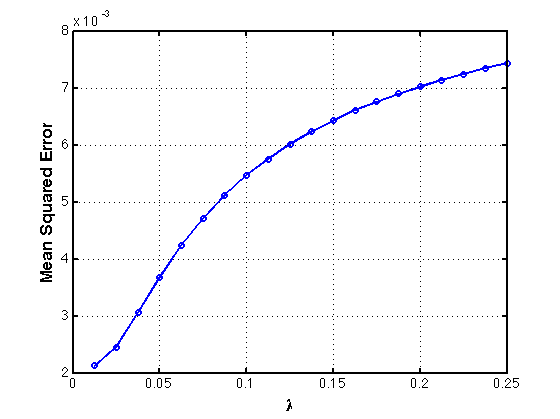
\includegraphics[width=\textwidth]{hemse.png}
                    \caption{MSE-$\lambda$}
					\end{subfigure}
					\begin{subfigure}{0.49\textwidth}
					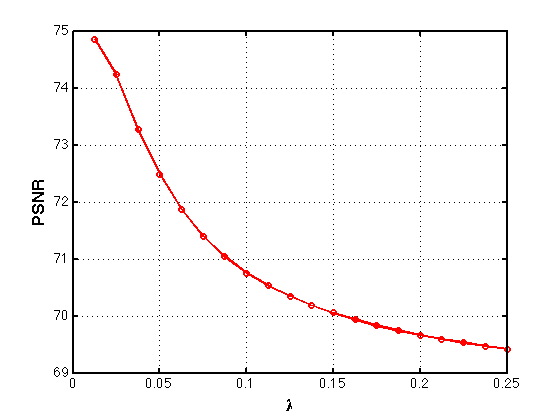
\includegraphics[width=\textwidth]{hepsnr.png}
                    \caption{PSNR-$\lambda$}
					\end{subfigure}
				\caption{MSE and PSNR for Heat Equation}
			\end{figure}
            \begin{figure}[H]
				\centering
				\begin{subfigure}{0.325\textwidth}
					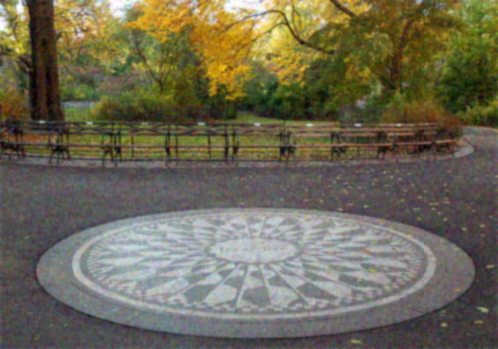
\includegraphics[width=\textwidth]{he1.png}
					\caption{$\lambda$=0.0125}
				\end{subfigure}
				\begin{subfigure}{0.325\textwidth}
					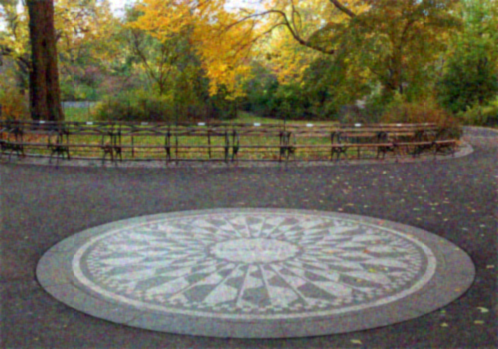
\includegraphics[width=\textwidth]{he3.png}
					\caption{$\lambda$=0.0375}
				\end{subfigure}
				\begin{subfigure}{0.325\textwidth}
					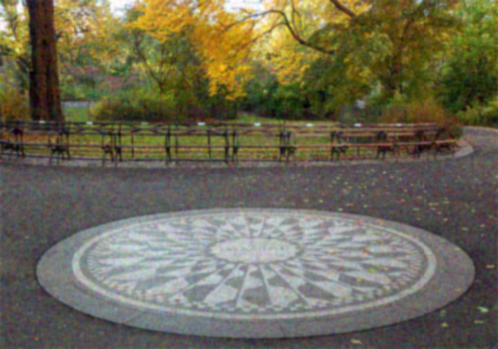
\includegraphics[width=\textwidth]{he8.png}
					\caption{$\lambda$=0.1000}
				\end{subfigure}
				\begin{subfigure}{0.325\textwidth}
					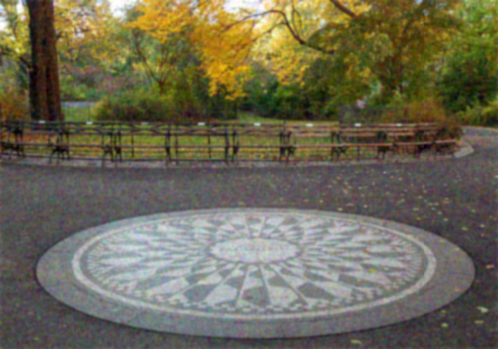
\includegraphics[width=\textwidth]{he11.png}
					\caption{$\lambda$=0.1375}
				\end{subfigure}
				\begin{subfigure}{0.325\textwidth}
					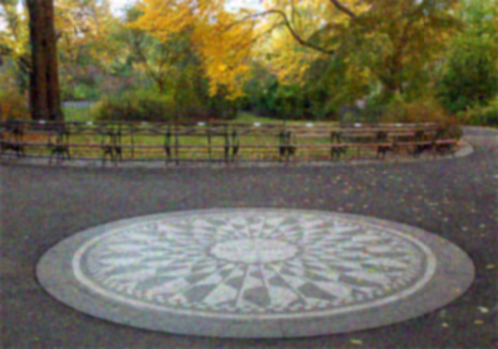
\includegraphics[width=\textwidth]{he16.png}
					\caption{$\lambda$=0.2000}
				\end{subfigure}
				\begin{subfigure}{0.325\textwidth}
					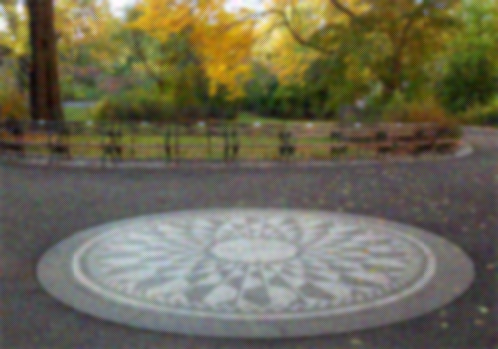
\includegraphics[width=\textwidth]{he20.png}
					\caption{$\lambda$=0.2500}
				\end{subfigure}
				\caption{Heat Equation with 6 different $\lambda$}
			\end{figure}
            \begin{figure}[H]
				\centering
				\begin{subfigure}{0.325\textwidth}
					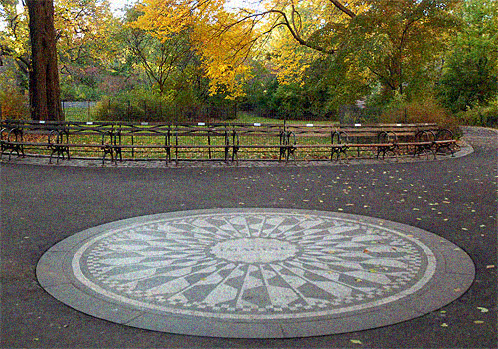
\includegraphics[width=\textwidth]{heat4.png}
					\caption{T=4}
				\end{subfigure}
				\begin{subfigure}{0.325\textwidth}
					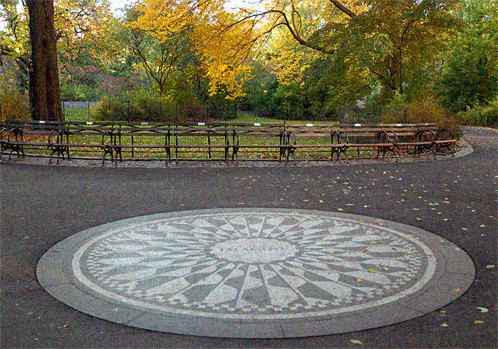
\includegraphics[width=\textwidth]{heat16.png}
					\caption{T=16}
				\end{subfigure}
				\begin{subfigure}{0.325\textwidth}
					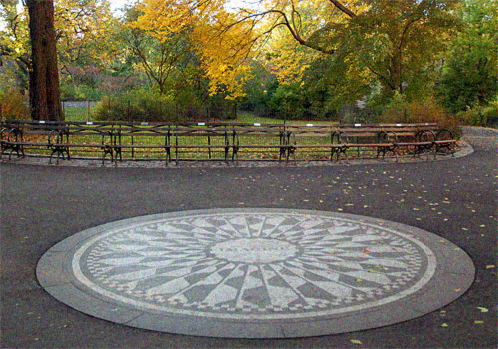
\includegraphics[width=\textwidth]{heat24.png}
					\caption{T=24}
				\end{subfigure}
				\begin{subfigure}{0.325\textwidth}
					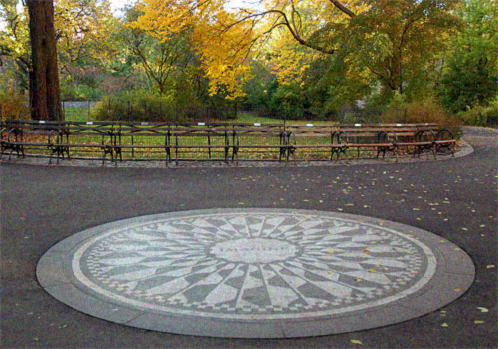
\includegraphics[width=\textwidth]{heat40.png}
					\caption{T=40}
				\end{subfigure}
				\begin{subfigure}{0.325\textwidth}
					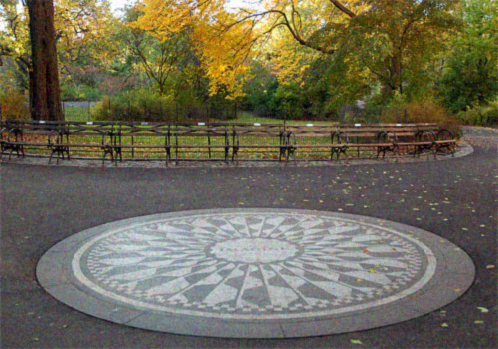
\includegraphics[width=\textwidth]{heat56.png}
					\caption{T=56}
				\end{subfigure}
				\begin{subfigure}{0.325\textwidth}
					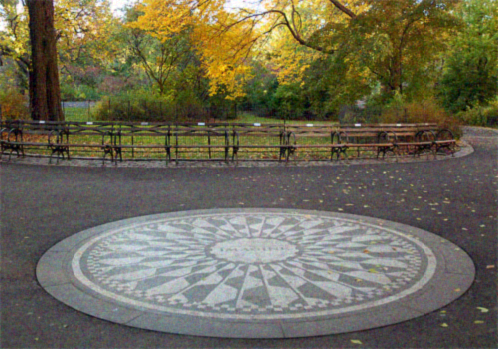
\includegraphics[width=\textwidth]{heat64.png}
					\caption{T=64}
				\end{subfigure}
		\caption{Heat Equation with 6 different time and fixed value $\lambda$=.00125}
			\end{figure}
For this project, steady state heat equation is used. This means that the PDE runs until the stopping condition is satisfied. For small number $\epsilon$, the following stopping condition is used:
%For this experiment, steady state of heat equation is used. That means that the PDE is running until the following stopping condition is satisfied.where $\epsilon$ is small positive number.
			\begin{alignat*}{1}
            \epsilon &< \min(\max(u_{i+1,j}+u_{i-1,j}+u_{i,j+1}+u_{i,j-1}-4u_{i,j}))
            \end{alignat*}
PSNR is upper bounded by approximately 75 and lower bounded by approximately 69. A Figure 3.2 (f) looks smoother than the other images of Figure 3.2. However, because the gap between upper and lower bound of PSNR for heat equation is approximately 6, there's no remarkable image restoration between Figure 3.2 (a) and (f). Figure 3.3 shows image restoration under same $\lambda$ but different time.
			%%%%%%%%%%%%%%%%%%%%%%%%%%%%%%%%%%%%%%%%%%%%%%%
			\section{Denoising with the Perona-Malik model}
			%%%%%%%%%%%%%%%%%%%%%%%%%%%%%%%%%%%%%%%%%%%%%%%
Recall that the conduction coefficients of the Perona-Malik equation can be determined in two ways: exponential and fractional. In this section, only denoising will be focused on.
			\begin{figure}[H]
				\centering
				\begin{subfigure}{0.49\textwidth}
				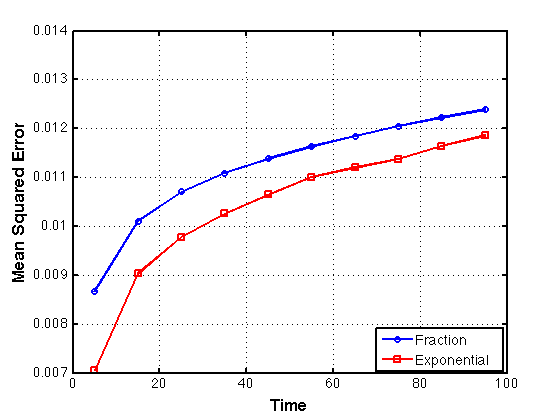
\includegraphics[width=\textwidth]{pmmse.png}
				\caption{MSE$-$Time}
				\end{subfigure}
				\begin{subfigure}{0.49\textwidth}
				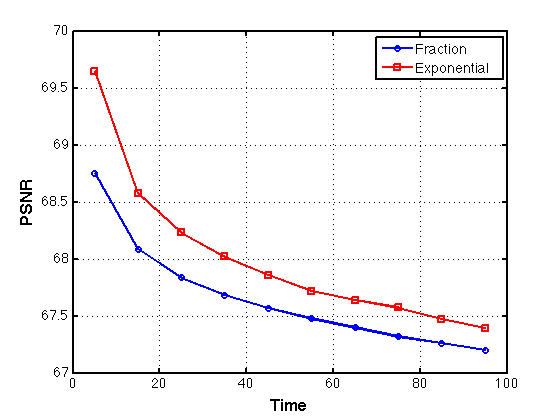
\includegraphics[width=\textwidth]{pmpsnr.png}
				\caption{PSNR$-$Time}
				\end{subfigure}
				\caption{MSE and PSNR for Perona-Malik model}
			\end{figure}
\noindent
The MSE graph above strictly increases, while PSNR graph strictly decreases. In MSE$-$time graph, the first exponential step is almost zero value. MSE value sits between 0.0007 and 0.0013. Time starts from 5 to 95 with step size 10.
            %%%%%%%%%%%%%%%%%%%%%%%%%%%%%%%%%%%%%%%%%%%%%%%%%%
			\subsection{Denoising with Fractional Coefficient}
            %%%%%%%%%%%%%%%%%%%%%%%%%%%%%%%%%%%%%%%%%%%%%%%%%%
%Note that $\lambda$=0.0125 specifies the first step of the process. As indicated by the graph above, denoising, with Fractional Coefficient of the first step, has a MSE value of approximately 0.002, which is close to zero. Furthermore, PSNR is approximately 69, and it seems that the image has been successfully restored, as shown by its clear edges and barely detectable noises. When $\lambda$=0.025, Figure 3.5 (b), the image starts to appear cartoonized and the edges become much smoother. These two images above are in the gray highlighted zone in the MSE$-\lambda$ graph. MSE value in the gray zone sits between 0.01 and 0.012, and the image that is in the gray zone looks similar.
There's a little difference between original noisy image and restored image which is executed during five time units. When time=15, it is distinguishable with noisy image (a). Figure (d) and (e) become more smoother than (b) and (c). Last, figure (f) results too smoother image so that some details that should be on the circle are wiped out.
            \begin{figure}[H]
				\captionsetup[subfigure]{labelformat=empty}
				\centering
				\begin{subfigure}{0.325\textwidth}
					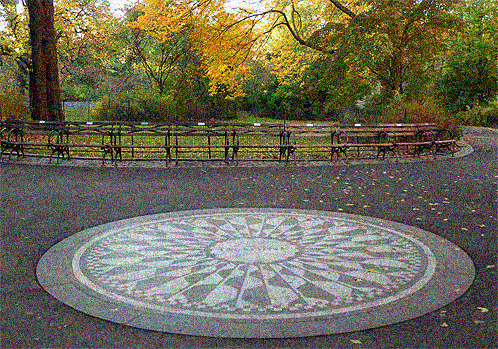
\includegraphics[width=\textwidth]{fractionnoise.png}
					\caption{(a) noisy image}
				\end{subfigure}
				\begin{subfigure}{0.325\textwidth}
					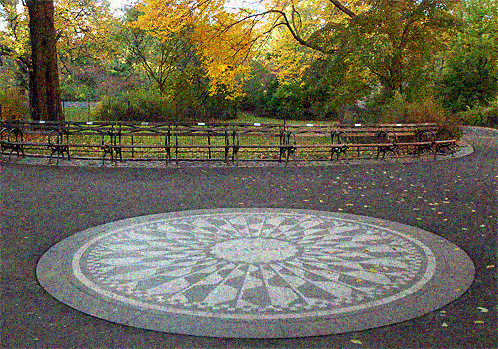
\includegraphics[width=\textwidth]{fraction5.png}
					\caption{(b) time=5}
				\end{subfigure}
				\begin{subfigure}{0.325\textwidth}
					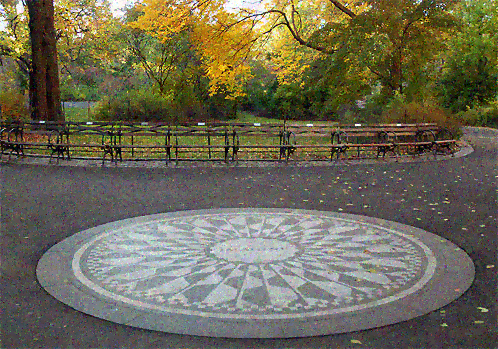
\includegraphics[width=\textwidth]{fraction15.png}
					\caption{(c) time=15}
				\end{subfigure}
		\caption{Images for Fractional Coefficients with time=5,15, and noisy image}
            \end{figure}
            \begin{figure}[H]
				\captionsetup[subfigure]{labelformat=empty}
				\begin{subfigure}{0.325\textwidth}
					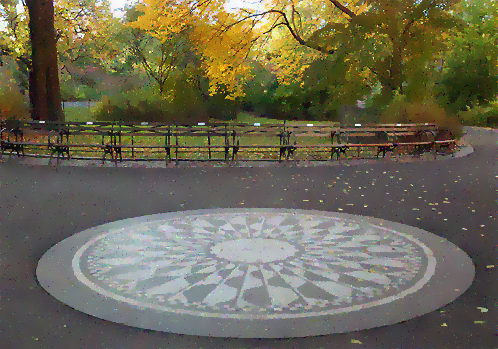
\includegraphics[width=\textwidth]{fraction35.png}
					\caption{(d) time=35}
				\end{subfigure}
				\begin{subfigure}{0.325\textwidth}
					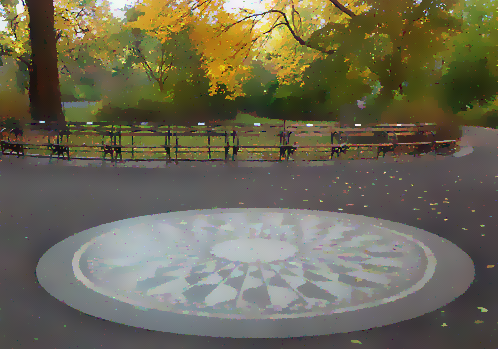
\includegraphics[width=\textwidth]{fraction55.png}
					\caption{(e) time=55}
				\end{subfigure}
				\begin{subfigure}{0.325\textwidth}
					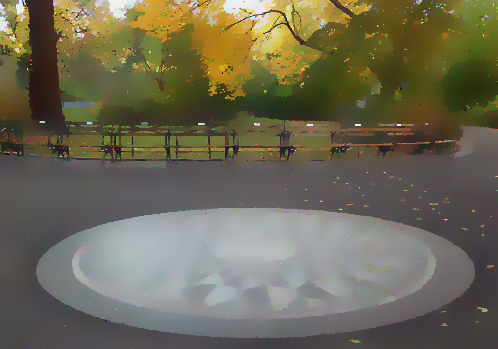
\includegraphics[width=\textwidth]{fraction95.png}
					\caption{(f) time=95}
				\end{subfigure}
		\caption{Images for Fractional Coefficients with time=35, 55, and 95}
			\end{figure}
            %%%%%%%%%%%%%%%%%%%%%%%%%%%%%%%%%%%%%%%%%%%%%%%%%%%
			\subsection{Denoising with Exponential Coefficient}
            %%%%%%%%%%%%%%%%%%%%%%%%%%%%%%%%%%%%%%%%%%%%%%%%%%%
Comparing (a) with (b) below, there's no remarkable difference between them. In MSE graph, it can be seen that the exponential line starts at almost zero. This is related with the fact that when two given images are identical, the MSE value will be zero. When time=15, the image is distinguished from noisy image. Figure 3.4 (b) shows that the PSNR values of exponential are larger in the entire time domain. From images (d), (e), and (f), it can be seen that as the time gets longer, smoothness is improved. The half of the details on the circle are wiped out when time=95.
%Comparing (a) with (b) below, there's no remarkable differences between them. In MSE graph, we can see that exponential line starts at almost zero. This is related with the fact that when two given images are identical, the MSE value will be zero. When time=15, the image is distinguished from noisy image. Figure 3.4 (b) shows that exponential's PSNR values are bigger in entire time domain. From images (d), (e), and (f), they are shown that as time gets longer, smoothness is much more improved. The half of details on the circle are wiped out when time=95.
			\begin{figure}[H]
				\centering
				\begin{subfigure}{0.325\textwidth}
					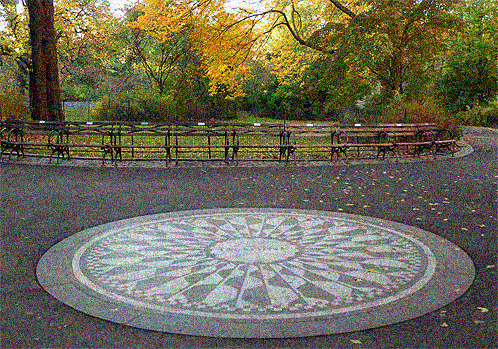
\includegraphics[width=\textwidth]{fractionnoise.png}
					\caption{noisy image}
				\end{subfigure}
				\begin{subfigure}{0.325\textwidth}
					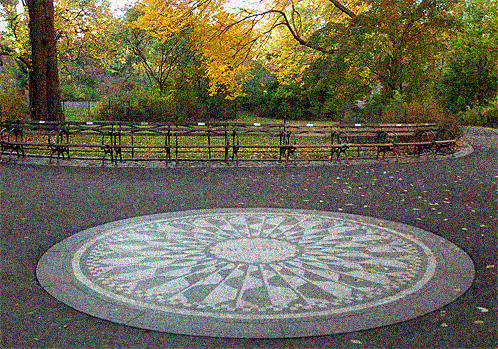
\includegraphics[width=\textwidth]{expo5.png}
					\caption{time=5}
				\end{subfigure}
				\begin{subfigure}{0.325\textwidth}
					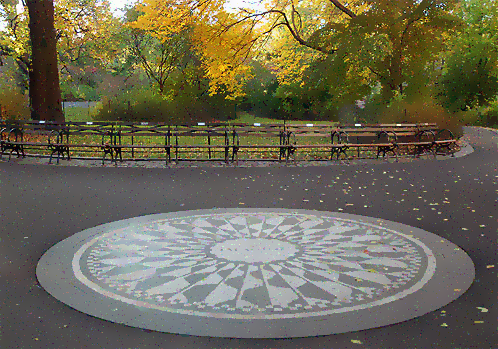
\includegraphics[width=\textwidth]{expo15.png}
					\caption{time=15}
				\end{subfigure}
				\begin{subfigure}{0.325\textwidth}
					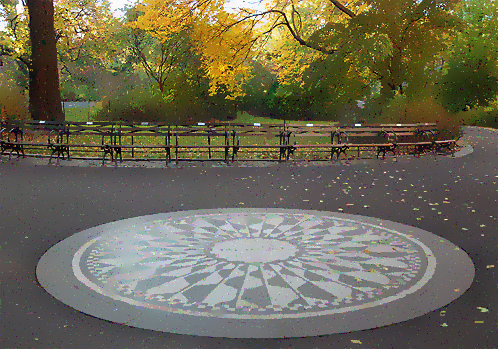
\includegraphics[width=\textwidth]{expo35.png}
					\caption{time=35}
				\end{subfigure}
				\begin{subfigure}{0.325\textwidth}
					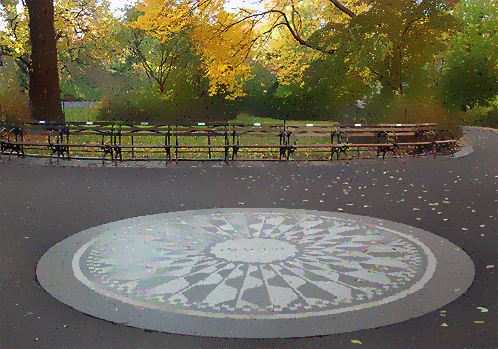
\includegraphics[width=\textwidth]{expo55.png}
					\caption{time=55}
				\end{subfigure}
				\begin{subfigure}{0.325\textwidth}
					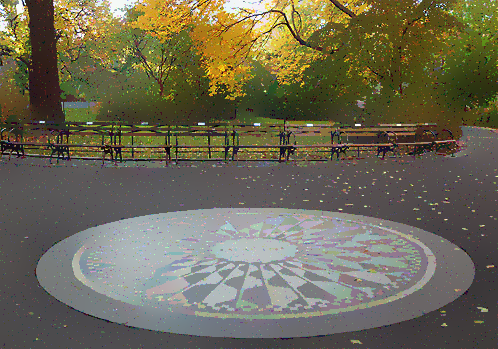
\includegraphics[width=\textwidth]{expo95.png}
					\caption{time=95}
				\end{subfigure}
		\caption{Images for Exponential Coefficients with five different execution time}
			\end{figure}
			%%%%%%%%%%%%%%%%%%%%%%%%%
            \section{Total variation}
			%%%%%%%%%%%%%%%%%%%%%%%%%
			\begin{figure}[H]
				\centering
				\begin{subfigure}{0.49\textwidth}
				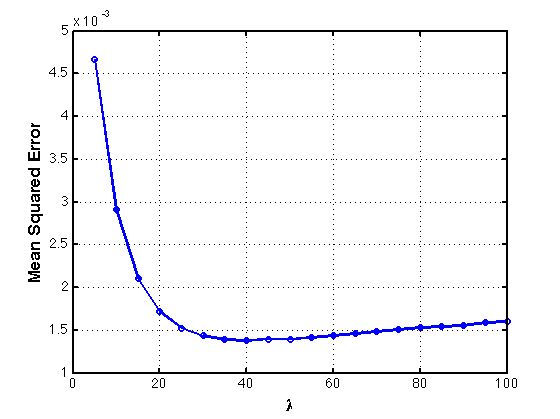
\includegraphics[width=\textwidth]{tv_mse.png}
				%\caption{Denoise SNR}
				\end{subfigure}
				\begin{subfigure}{0.49\textwidth}
				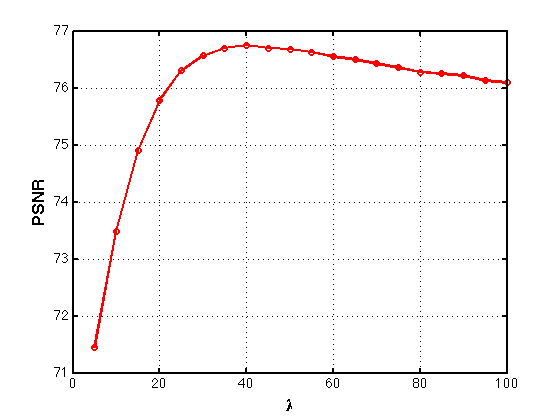
\includegraphics[width=\textwidth]{tv_psnr.png}
				%\caption{Blur SNR}
				\end{subfigure}
				\caption{MSE and PSNR for the total variation}
			\end{figure}
MSE hits the minimum at between $\lambda$=35 and 40. It implies that PSNR hits the maximum values in that interval. After reaching the maximum PSNR value, the graph starts to decrease and approaches to value of 76. This shows that once PSNR approaches the maximum value, the restored images are likely to become noisy (a). Figure 3.10 (d) is the restored image when PSNR has its maxima. $\lambda$ less than 5 is also applied and is shown below in Figure 3.10 (b). When $\lambda$=0.25, the image is too smooth for objects in the picture to be distinguished.
            \begin{figure}[H]
				\centering
				\begin{subfigure}{0.325\textwidth}
					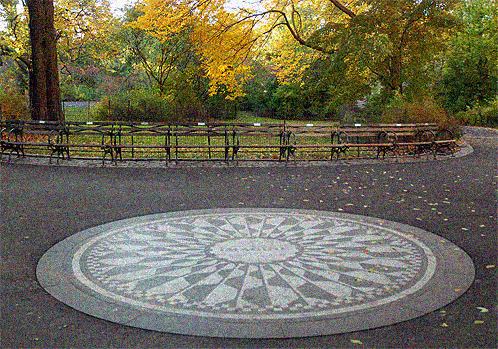
\includegraphics[width=\textwidth]{tvnoise.png}
					\caption{Noisy image}
				\end{subfigure}
				\begin{subfigure}{0.325\textwidth}
					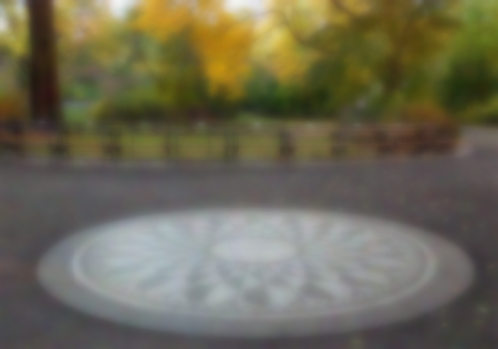
\includegraphics[width=\textwidth]{tv_quarter.png}
					\caption{$\lambda$=0.25}
				\end{subfigure}
				\begin{subfigure}{0.325\textwidth}
					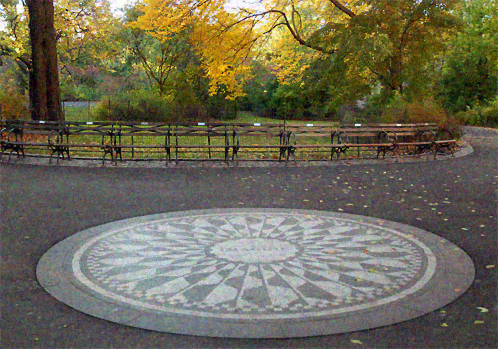
\includegraphics[width=\textwidth]{tv20.png}
					\caption{$\lambda$=20}
				\end{subfigure}
				\begin{subfigure}{0.325\textwidth}
					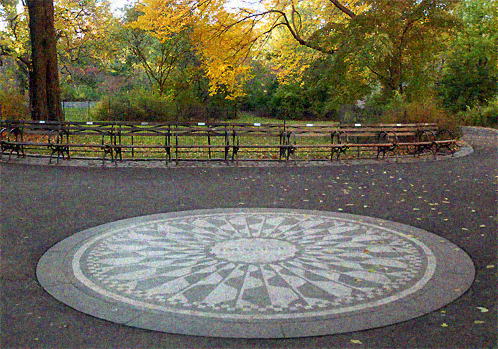
\includegraphics[width=\textwidth]{tv40.png}
					\caption{$\lambda$=40}
				\end{subfigure}
				\begin{subfigure}{0.325\textwidth}
					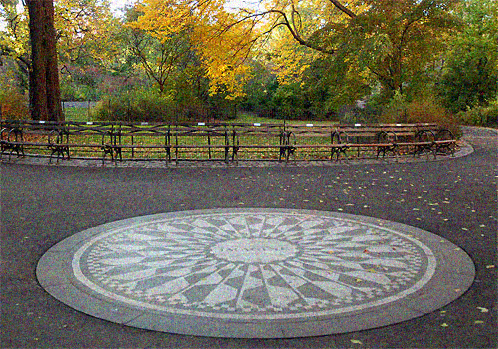
\includegraphics[width=\textwidth]{tv80.png}
					\caption{$\lambda$=80}
				\end{subfigure}
				\begin{subfigure}{0.325\textwidth}
					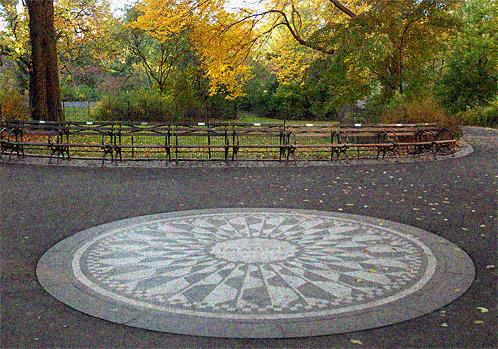
\includegraphics[width=\textwidth]{tv100.png}
					\caption{$\lambda$=100}
				\end{subfigure}
                \caption{Denoise depends on $\lambda$}
			\end{figure}
			\begin{figure}[H]
				\centering
				\begin{subfigure}{0.49\textwidth}
				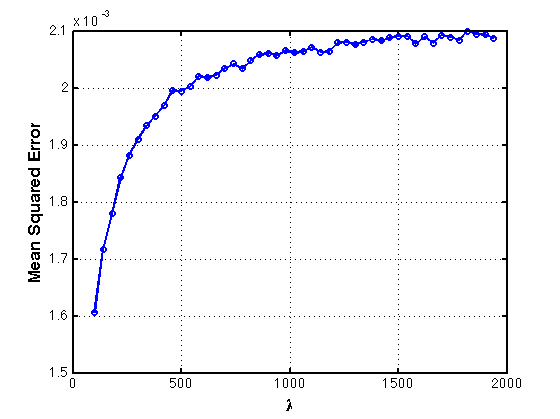
\includegraphics[width=\textwidth]{tvmseextra.png}
				\end{subfigure}
				\begin{subfigure}{0.49\textwidth}
				\includegraphics[width=\textwidth]{tvpnsrextra.png}
				\end{subfigure}
				\caption{MSE and PSNR for the large $\lambda$}
			\end{figure}
\noindent
%Figure 3.10 show how PSNR behaves when $\lambda$ gets bigger than 100. PSNR looks descreasing but not monotonically descreasing and it converges to approximately 74.5.
Figure 3.11 shows how PSNR behaves when $\lambda$ becomes larger than 100. PSNR is decreasing but not monotonically decreasing and it finally converges to approximately 74.5.
        % ---------- %
        % CONCLUSION %
        % ---------- %
		\chapter{Conclusion}
In this work, we studied how the machine recognizes digital image and the image can be processed. Because humans have a sensitive eye, not only performing image processing but also finding image quality are important. PSNR and MSE are introduced as measurements of image quality. PSNR is defined as follows:
%In this work, we studied how the machine recognize digital image and how image can be processed. Because human has a sensitve eye, not only performing image processing but also finding image quality are important. PSNR and MSE are introduced as a measurements of image quality. PSNR is defined as follows:
			\begin{alignat*}{1}
\displaystyle PSNR &= 20\log\big({MAX_{I}}\big) - 10\log\big(MSE\big)
	        \end{alignat*}
\par
The higher PSNR implies better image quality. Hence, the PSNR is directly related with the quality of the image. In \textbf{Chapter 3}, we have shown the MSE and PSNR values for each algorithms.
%Recall that higher PSNR implies better image quality. They have disproportional relationship. In \textbf{Chapter 3}, we have shown the following MSE and PSNR values for each algorithms.
%\begin{table}[h]
\begin{center}
\begin{tabular}{@{}lllll@{}}
\toprule
\multicolumn{1}{c}{} 	& \multicolumn{1}{c}{MSE} & \multicolumn{1}{c}{PSNR} &  &  \\ \midrule
\multicolumn{1}{c}{Heat equation}   & \multicolumn{1}{c}{71-77} & \multicolumn{1}{c}{0.001-0.045} &  &  \\
\multicolumn{1}{c}{Perona-Malik}    & \multicolumn{1}{c}{67-70} & \multicolumn{1}{c}{0.007-0.012} &  &  \\
\multicolumn{1}{c}{Total Variation} & \multicolumn{1}{c}{69-75} & \multicolumn{1}{c}{0.002-0.006} &  &  \\ \bottomrule
\end{tabular}
\end{center}
%\end{table}
\par
%Following two images (b) and (c) are restored by Perona-Malik anisotropic diffusion equation with time=20. These two are best results during the entire image processing work, because the noises are clearly removed and the image (b) keeps the sharp edges.
Following two images give the figure number as well here (b) and (c) are restored by Perona-Malik anisotropic diffusion equation with time=20. These two are best results during the entire image processing work, because the noises are clearly removed and the image give the figure number as well here (b) has sharp edges. Among the restored images in \textbf{Chapter 3}, even PSNR and MSE show that the shown images are restored from noise. There are still a few yellowish or reddish dots, especially around the circle, which occur because the color conversion between RGB and YUV has not been applied.
			\begin{figure}[H]
				\centering
				\begin{subfigure}{0.325\textwidth}
					\includegraphics[width=\textwidth]{fractionnoise.png}
                    \caption{Noisy image}
				\end{subfigure}
				\begin{subfigure}{0.325\textwidth}
					\includegraphics[width=\textwidth]{pm1.png}
                    \caption{$\mu$=0.0125}
				\end{subfigure}
				\begin{subfigure}{0.325\textwidth}
					\includegraphics[width=\textwidth]{pm2.png}
                   	\caption{$\mu$=0.025}
				\end{subfigure}
				\caption{Two best results by Perona-Malik anisotropic diffusion equation}
			\end{figure}
\par
Among the restored images in \textbf{Chapter 3}, even PSNR and MSE tell that the shown images are restored from noise, there's still a few yellowish or reddish dots around the circle especially. It occurred because color conversion between RGB and YUV has not been applied.
\newline
\par

	\end{tableofcontents}
\renewcommand{\bibname}{References}
\bibliographystyle{plain}
\bibliography{scholar.bib}

\end{document}




%-------------------------------
%-------------------------------
\iffalse
\newline
\par
In the following paragraphs, I will discuss the structure that these images possess in the matrix, and the color responding value ranges that images hold as entries of a matrix. For example, grayscale and true color images(RGB) have different matrix structures. Suppose we have an $M\times N\times n$ size image. Grayscale uses an $M\times N$ form of two dimensional matrix with $n$=1, while true color image uses an $M\times N\times$3 form of three dimensional matrix. $M$ and $N$ represent the pixel coordinates, while the third index of a true color images represents its color channel.
\fi
%-------------------------------
%-------------------------------



%%%%%%% DONE WITH GRAMMAR UNTIL HERE !!!!!!
%%%%%%% as of December 14 !!!!!!!!!!!!!!!!!
%------------------------------------
%------------------------------------
\iffalse
Let $v$ be the directional function. The first variation of energy function (2.1) is given by
			\begin{alignat*}{3}
\displaystyle\frac{d}{dt}\Biggm|_{t=0}E[u+tv]
&= \frac{1}{2} \int_{\Omega}\frac{d}{dt}\Biggm|_{t=0}\Big[\phi(|\nabla u + t\nabla v|^{2})
        + \lambda(u+tv-f)^{2}\,\Big] dx dy \\
&= \frac{1}{2} \int_{\Omega}2\phi'(|\nabla u|^{2})\nabla u\nabla v
		+ 2\lambda(u+tv-f)(v)\,dx dy \\
&= \int_{\Omega}\Big[ \text{div}(\phi'(|\nabla u|^{2}\nabla u) + \lambda(u-f)\Big]v\, dx dy
		+ \int_{\Omega}\phi'(|\nabla u|^{2})
        \underbrace{\nabla u\cdot\hat{n}}_{=0} \, dx dy
            \end{alignat*}
Therefore, the gradient is given that
			\begin{alignat*}{1}
\nabla_{L^{2}}E[u] &= -\text{div}\Big( \phi'(|\nabla u|^{2})\nabla u\Big)
            \end{alignat*}
Furthemore, the gradient descent
			\begin{equation}
\frac{\partial u}{\partial t}
	= \text{div}\Big( \phi'(|\nabla u|^{2})\nabla u\Big) + \lambda (f-u)
            \end{equation}
\fi
%------------------------------------
%------------------------------------
%--------------------------------------------
%--------------------------------------------
%--------------------------------------------
\iffalse
define function $E\left[u\right]$ as follows
				\begin{equation}
                E\left[u\right] = \text{min}\int_{\Omega}|\nabla u|^{2}dxdy
                \end{equation}
The way to approach is to find the minimize of (2.2), then evolve heat equation. First of all, introduce function $g(u, u_{x}, u{y}) = |\nabla u|^{2} = u_{x}^{2} + u_{y}^{2}$. Now it has a functional of the form,
				\begin{alignat*}{1}
                E\left[u\right] &= \int_{\Omega}g(u, u_{x}, u_{y})
                \end{alignat*}
By Euler-Lagrange equation for $\nabla E$,
				\begin{alignat*}{3}
\displaystyle\nabla E &= \frac{\partial g}{\partial u}
			- \frac{\partial}{\partial x}\frac{\partial g}{\partial u_{x}}
            - \frac{\partial}{\partial y}\frac{\partial g}{\partial u_{y}} \\
         &= 0 - \frac{\partial}{\partial x}2u_{x}
              - \frac{\partial g}{\partial y}2u_{y}  \\
         &= -2u_{xx} - 2u_{yy} \\
         &= -2\Delta u
				\end{alignat*}
\fi
%--------------------------------------------
%--------------------------------------------
%--------------------------------------------
%The heat equation was first used in image processing and computer vision by Witkin \cite{witkin}. For the heat equation $\frac{\partial u}{\partial t} = \Delta u$, we have $\phi(s) = s$.
%assume that $dt$ be the small time step and find the minimum of $E\left[u\right]$, we have
%				\begin{equation}
%                u_{i,j}^{n+1} = u_{i,j}^{n} + \Delta t(-\nabla E) \\
%                			  \approx u_{i,j}^{n} + \Delta t\Delta u + \lambda(f_{i.j}-u_{i,j})
%                \end{equation}
%Note that gradient descent on $E$ is
%				\begin{equation}
 %               \frac{\partial u}{\partial t} = \nabla u%- \nabla_{L^2}E(u)
  %              \end{equation}
%Combining (2.1) and (2.2),
%				\begin{equation}
%                \frac{\partial u}{\partial t} = \Delta u  + \lambda(f-u)
%                \end{equation}
%Note that Laplacian of $u(x,y)$ is defined by
%				\begin{alignat*}{1}
%\displaystyle\Delta u &= \frac{\partial^2 u}{\partial x^2} + \frac{\partial^2 u}{\partial y^2}
%                \end{alignat*}

%As Pascal Getreuer introduced, when $u$ is smooth, TV is equivalently the integral of its gradient magnitude,
%				\begin{alignat*}{1}
%                \displaystyle||u||_{TV(\Omega)} &= \int_{\Omega}|\nabla u| dx
%                \end{alignat*}
%where $\displaystyle||u||_{TV(\Omega)} \approx \sum_{i,j} \sqrt{(\nabla_{x}u)_{i,j}^{2} + (\nabla_{y}u)_{i,j}^{2}}$.
%\newline
%--------------------------------------------
%--------------------------------------------
%--------------------------------------------
\iffalse
Introduce total variation denoising by gradient descent,
				\begin{equation}
                \frac{\partial u}{\partial t} = -\nabla E
                \end{equation}
Let $v(x,y)$ be the directional function. Then take the following
				\begin{alignat*}{7}
\frac{d}{dt}\biggm |_{t=0} \int_{\Omega}\Big(|\nabla u + t\nabla v|\Big)dx
% &= \frac{d}{dt}\biggm |_{t=0} \int_{\Omega}|\nabla u + t\nabla v| dx \\
 &= \int_{\Omega}\frac{d}{dt}\biggm |_{t=0}\sqrt{
 		\Big(\frac{\partial u}{\partial x} + t\frac{\partial v}{\partial x}\Big)^{2}
          + \Big(\frac{\partial u}{\partial y} + t\frac{\partial v}{\partial y}\Big)^{2}}dxdy \\
 &= \int_{\Omega}\Big[
 					 \Big(\frac{\partial^{2} u}{\partial x^{2}}
 							+ \frac{\partial^{2} u}{\partial y^{2}}\Big)^{-\frac{1}{2}}
                     \Big(\frac{\partial u}{\partial x}
                     + t\frac{\partial v}{\partial x}\Big)\frac{\partial v}{\partial x} \\
               &\qquad + \Big(\frac{\partial^{2} u}{\partial x^{2}}
 							+ \frac{\partial^{2} u}{\partial y^{2}}\Big)^{-\frac{1}{2}}
   					 \Big(\frac{\partial u}{\partial y}
   							+t\frac{\partial v}{\partial y}\Big)\frac{\partial v}{\partial y}
                      \Big]_{t=0}dxdy \\
 &= \int_{\Omega}\frac{1}{|\nabla u|}\Big(\frac{\partial u}{\partial x}\frac{\partial v}{\partial x}
 				+ \frac{\partial u}{\partial y}\frac{\partial v}{\partial y}
                                   \Big)dxdy \\
 &= \int_{\Omega}\Big(\frac{\nabla u}{|\nabla u|}\Big)\cdot\nabla v\cdot dxdy \\
 &= \left< \nabla_{{L}^{2}} E(u), v\right>
                \end{alignat*}
\newline
From the last equation above, we define $L^{2}$ as described above. By integration by parts,
				\begin{alignat*}{1}
\left< \nabla_{{L}^{2}} E(u), v\right>
 &= -\int_{\Omega}\text{div}\Big(\frac{\nabla u}{|\nabla u|}\Big)\cdot\nabla v dx
		+ \int_{\Omega}\frac{\nabla u}{|\nabla u|}\cdot\hat{n} v dx \\
 &= \left<-\text{div}\Big(\frac{\nabla u}{|\nabla u|}\Big), v\right>
                \end{alignat*}
where we set $\frac{\partial u}{\partial\hat{n}}= 0$. %= D$u\cdot\hat{u}$ = 0
\newline
\newline
\fi
%--------------------------------------------
%--------------------------------------------
%--------------------------------------------
%Suppose $u$ be the restored and $f$ be the corrupted image by noise.
%The equation (2.5) yields $\Delta t\Delta u$ of (2.3). Thus, we can conclude that
%Let's apply prior term first. The equation (2.2) implies that $\partial u/\partial t = (u_{i,j}^{n+1}-u_{i,j}^{n})/\Delta t$ and this implies that
%Finally, adding fidelity term $\lambda(f-u)$ to last equation gives the complete form of heat equation
%				\begin{alignat*}{1}
%                \displaystyle u_{i,j}^{n+1} &= u_{i,j}^{n} + \Delta t\big(u_{i+1,j}+u_{i-1,j}+u_{i,j+1}+u_{i,j-1}-4u_{i,j}\big) + \lambda\big(f_{i,j}-u_{i,j}\big)
%                \end{alignat*}
\iffalse
            \begin{figure}[H]
				\centering
				\begin{subfigure}{0.49\textwidth}
					\includegraphics[width=\textwidth]{fractionnoise.png}
					\caption{$\lambda$=0.0125}
                \end{subfigure}
                \begin{subfigure}{0.49\textwidth}
					\includegraphics[width=\textwidth]{fractionnoise.png}
					\caption{Noisy Image}
				\end{subfigure}
				\begin{subfigure}{0.325\textwidth}
					\includegraphics[width=\textwidth]{fractionnoise.png}
					\caption{$\lambda$=0.05}
				\end{subfigure}
				\begin{subfigure}{0.325\textwidth}
					\includegraphics[width=\textwidth]{fractionnoise.png}
					\caption{$\lambda$=0.075}
				\end{subfigure}
				\begin{subfigure}{0.325\textwidth}
					\includegraphics[width=\textwidth]{fractionnoise.png}
					\caption{$\lambda$=0.125}
				\end{subfigure}
                \caption{Image on non gray zone}
            \end{figure}
            \begin{figure}[H]
				\centering
				\captionsetup[subfigure]{labelformat=empty}
				\begin{subfigure}{0.49\textwidth}
					\includegraphics[width=\textwidth]{fractionnoise.png}
					\caption{(a) $\lambda$=0.1875}
				\end{subfigure}
				\begin{subfigure}{0.49\textwidth}
					\includegraphics[width=\textwidth]{fractionnoise.png}
					\caption{(b) $\lambda$=0.25}
				\end{subfigure}
                \caption{Image on gray zone}
			\end{figure}
%In Figure 3.6, first step image has approximately zero MSE value. Hence, noise is not completely wiped out. Figure 3.7, Similar with previous sub section, $\lambda$=0.05 results best one among non gray zone images. As $\lambda$ approaches to 0.125, the edges become more smoother. Figure 3.8, The gray zone results too smooth images as we've already shown previously.
            %%%%%%%%%%%%%%%%%%%%%%%%%%%%%%%%%%%%%%%%%%%%%%%%%%%%%%%%%%%%%%
            \section{Perona-Malik to Deblur in two different coefficients}
            %%%%%%%%%%%%%%%%%%%%%%%%%%%%%%%%%%%%%%%%%%%%%%%%%%%%%%%%%%%%%%
			\begin{figure}[H]
				\centering
				\begin{subfigure}{0.49\textwidth}
				\includegraphics[width=\textwidth]{blur_mse_update.png}
				\end{subfigure}
				\begin{subfigure}{0.49\textwidth}
				\includegraphics[width=\textwidth]{blur_psnr.png}
				\end{subfigure}
				\caption{MSE and PSNR for Deblurring Image Processing}
			\end{figure}
%Regardless of type of coefficients, the first image with smallest K give us more clearer than other five images. In MSE$-\lambda$ graph, here's a gray highlighted zone that contains all the point that MSE is greater than 0.0016. Then in two or three steps, the MSE value converges to near 0.0016. Therefore, if the step value $\lambda$ is greater than 0.05(Fractional) and 0.0625(Exponential), not remarkable change occurred.
Regardless of the type of coefficients, the first image, with the smallest K value, gives us an image much clearer than the other five. In the MSE$-\lambda$ graph, we see a gray highlighted zone that contains all the points where the MSE is greater than 0.0016. Then, in two or three steps, the MSE value converges to 0.0016. Therefore, no remarkable changes have occurred when the step value $\lambda$ is greater than 0.05(Fractional) or 0.0625(Exponential).
            %%%%%%%%%%%%%%%%%%%%%%%%%%%%%%%%%%%%%%%%%%%%%%%%%%%
			\subsection{Deblurring with Fractional coefficient}
            %%%%%%%%%%%%%%%%%%%%%%%%%%%%%%%%%%%%%%%%%%%%%%%%%%%
            \begin{figure}[H]
				\centering
				\captionsetup[subfigure]{labelformat=empty}
				\begin{subfigure}{0.32\textwidth}
					\includegraphics[width=\textwidth]{pmb1.png}
					\caption{$\lambda$=0.0125}
				\end{subfigure}
				\begin{subfigure}{0.32\textwidth}
					\includegraphics[width=\textwidth]{pmb3.png}
					\caption{$\lambda$=0.0375}
				\end{subfigure}
				\begin{subfigure}{0.32\textwidth}
					\includegraphics[width=\textwidth]{pmb4.png}
					\caption{$\lambda$=0.05}
				\end{subfigure}
				\begin{subfigure}{0.32\textwidth}
					\includegraphics[width=\textwidth]{pmb10.png}
					\caption{$\lambda$=0.125}
				\end{subfigure}
				\begin{subfigure}{0.32\textwidth}
					\includegraphics[width=\textwidth]{pmb16.png}
					\caption{$\lambda$=0.20}
				\end{subfigure}
				\begin{subfigure}{0.32\textwidth}
					\includegraphics[width=\textwidth]{pmb20.png}
					\caption{$\lambda$=0.25}
				\end{subfigure}
			\end{figure}
            %%%%%%%%%%%%%%%%%%%%%%%%%%%%%%%%%%%%%%%%%%%%%%%%%%%%
			\subsection{Deblurring with Exponential Coefficient}
            %%%%%%%%%%%%%%%%%%%%%%%%%%%%%%%%%%%%%%%%%%%%%%%%%%%%
            \begin{figure}[H]
				\centering
				\captionsetup[subfigure]{labelformat=empty}
				\begin{subfigure}{0.32\textwidth}
					\includegraphics[width=\textwidth]{pmbe1.png}
					\caption{$\lambda$=0.0125}
				\end{subfigure}
				\begin{subfigure}{0.32\textwidth}
					\includegraphics[width=\textwidth]{pmbe3.png}
					\caption{$\lambda$=0.0375}
				\end{subfigure}
				\begin{subfigure}{0.32\textwidth}
					\includegraphics[width=\textwidth]{pmbe6.png}
					\caption{$\lambda$=0.075}
				\end{subfigure}
				\begin{subfigure}{0.32\textwidth}
					\includegraphics[width=\textwidth]{pmbe10.png}
					\caption{$\lambda$=0.125}
				\end{subfigure}
				\begin{subfigure}{0.32\textwidth}
					\includegraphics[width=\textwidth]{pmbe16.png}
					\caption{$\lambda$=0.20}
				\end{subfigure}
				\begin{subfigure}{0.32\textwidth}
					\includegraphics[width=\textwidth]{pmbe20.png}
					\caption{$\lambda$=0.25}
				\end{subfigure}
			\end{figure}
%Because MSE and PSNR gaps between exponential and fractional at each step is relatively small, the two sets in two different type of coefficients look similar.
Because the MSE and PSNR gaps between exponential and fractional are relatively small at each step, the two sets look similar in both types of coefficients.
\fi
%Therefore, the gradient descent is
%				\begin{alignat*}{1}
%\frac{\partial u}{\partial t} = \text{div}\Big(\frac{\nabla u}{|\nabla u|}\Big) + \lambda(f-u)
%				\end{alignat*}
%where $\partial u/\partial\hat{n} = 0$ , on $\partial\Omega\times\big[0, \infty\big)$.
%                \begin{figure}[t]
%				\centering
%				\begin{subfigure}{0.2\textwidth}
%					\includegraphics[width=\textwidth]{stencils.png}
%				\end{subfigure}
%				\caption{Eight stencils for Total Variation}
%               \end{figure}
%\newline \newline Note that for the rest of the paper, the solution for each PDE involves a step size of 0.0125 and a time T=20. Furthermore, the experimental parameter is $\lambda$.
%The images above are choosen at 3 maxima and minima points from MSE graph. However, the six images above look similar to each other. This is because the difference between maximum and minimum value of PSNR is approximately 0.5, which is small number when it comes to a logarithmic scale.
%Recall that the conduction coefficients of the Perona-Malik can be determined in two ways,namely exponential and fractional. In this section, we focus only on denoising.
%The graphs above strictly increasing but convergences to near MSE=0.001. In MSE-$\lambda$ graph, if coefficients is greater .05, MSE value is between 0.01 and 0.012. Denote gray zone be the gray highlighted area in Figure3.3.(a).
%Note that $\lambda$=0.0125 means the first step of the process. As indicated graph above, denoising with Fractional Coefficient of the first step is 0.002, which is close to zero. Furthermore, PSNR is approximately 65 and it seems that image has been successfully restored, because It has clear edges and barely find the noises. When $\lambda$=0.025, the image starts to be cartoonized and edges become more smoother.
%These two images above are in the gray highlighted zone in MSE$-\lambda$ graph. MSE value in gray zone is between 0.01 and 0.012, the image that in the gray zone looks similar.
%MSE is strictly decreasing while PSNR is strictly increasing. When $K$=0.25, the image is too smooth to distinguish objects in the picture. Thus, TV denoising application with $\lambda$=0.25 wouldn't give us better result amongst many options. Then now it is easy to see that image gets much better as K is increasing.
%MSE is strictly decreasing while PSNR is strictly increasing. When $\lambda$=0.25, the image is too smooth for objects in the picture to be distinguished. Thus, the TV denoising application with $\lambda$=0.25 wouldn't give us a better result amongst many other options. Now it is easier to see that the image gets much better as $\lambda$ increases.
%One of the largest challenges for me was writing and optimizing the mathematical schemes in Matlab code. Just as we have discussed how machines import digital images, the PDE schemes must be applied at every single point. This wouldn't cause any problems for smaller-sized images. However, for relatively large-sized images, this solution seems ineffective because it requires so much time to execute, and very few customers would be willing to wait for such a long while. Fortunately, Matlab provides many useful commands, such as \textbf{circshift}, \textbf{padarray}, and \textbf{del2}. The first command pads the given array, which helps with translating the matrix in four directions. The second command circularly shifts the entries in any direction the user wants. The last one returns the discrete Laplacian, which I didn't use for my paper. Using the first two commands, I can compute mathematical arithmetic matrix-wise. I spent much time writing the mathematical schemes in Matlab. If I used various Matlab-provided functions such as PSNR and MSE, I could have saved time. Thinking with respect to the future, I wish I had focused more on the algorithm, and more specifically the optimization of its parameters.
